% chapter1.tex -- Introduction
% Based on the author's UGThesis.docx and the Parvez-Rahman-Nakano paper.

\chapter{Introduction}
\label{ch:introduction}

\section{Motivation and Applications}
\label{sec:motivation}

The problem of generating all triangulations of plane graphs arises in many areas of computational geometry~\cite{berg2008}, VLSI floorplanning~\cite{kozminski1985}, and graph drawing~\cite{nishizeki2004}. 
A triangulation of a plane graph is a maximal set of non‑crossing chords that partition each face into triangles. 
Enumerating all possible triangulations is essential for exploring geometric configurations, optimizing layouts, and testing hypotheses about graph properties.

In VLSI design, for instance, different triangulations of a floorplan correspond to different routing possibilities. 
In mesh generation, enumerating triangulations helps to find optimal finite element meshes. 
In graph drawing, triangulations are used to create straight‑line embeddings and to study graph properties.

\section{Challenges in Generating All Triangulations}
\label{sec:challenges}

The number of triangulations of a planar graph can be exponential in the number of vertices. 
For a convex polygon with \(n\) vertices, the number of triangulations is the Catalan number \(C_{n-2}\), which grows as \(\Theta(4^n n^{-3/2})\). 
For general plane graphs, the count can be even larger. 
Therefore, any algorithm that lists all triangulations must handle an exponential output size.

The main challenges in designing such algorithms are threefold:
\begin{enumerate}
    \item \textbf{Exponential output:} The algorithm must run in time proportional to the number of triangulations; otherwise it would be inefficient.
    \item \textbf{Avoiding duplicates:} Since the output is huge, storing previously generated triangulations to check for duplicates would require exponential space and time.
    \item \textbf{Space efficiency:} The algorithm should use only polynomial space (preferably linear in the input size) and not store all outputs simultaneously.
\end{enumerate}

Classical approaches to generating combinatorial objects include orderly algorithms~\cite{mckay1998} and reverse search~\cite{avis1996}. 
Orderly algorithms generate objects in a canonical form and output only those that are canonical, thus avoiding duplicates without storing all previous objects. 
Reverse search defines a spanning tree on the graph of objects and traverses it using a parent function, again without storing the entire set.

\section{Previous Work}
\label{sec:previous_work}

There is a rich literature on triangulation enumeration. 
For convex polygons, it is well known that triangulations correspond to binary trees, and efficient generation algorithms exist that run in constant amortized time per triangulation~\cite{hurtado1999}. 

For planar graphs, the problem is more challenging. 
Li and Nakano~\cite{li2001} gave an algorithm to generate all biconnected plane triangulations with at most \(n\) vertices in \(O(r^2 n)\) time per triangulation, where \(r\) is the number of vertices on the outer face. 
Later, Nakano improved this to \(O(r n)\) time per triangulation.

The most relevant prior work is the algorithm by Parvez, Rahman, and Nakano~\cite{parvez2011}, which generates all triangulations of a \emph{triconnected} plane graph in \(O(1)\) amortized time per triangulation using \(O(n)\) space. 
This algorithm defines a genealogical tree of triangulations where each node is a triangulation and each edge corresponds to a chord flip. 
By traversing this tree in a depth‑first manner, all triangulations are generated without duplicates.

However, the algorithm of Parvez et al. is limited to triconnected graphs. 
As we will explain in Section~\ref{sec:limitation}, extending it directly to biconnected graphs leads to the multi‑edge problem caused by separation pairs. 
This limitation is the main motivation for our work.

\section{The Parvez–Rahman–Nakano 2011 Algorithm (Overview)}
\label{sec:parvez_overview}

We briefly recall the key ideas of the algorithm for triconnected plane graphs, as they form the foundation of our approach.

Given a triconnected plane graph \(G\) with \(n\) vertices, the algorithm processes all faces simultaneously. 
For each face \(F_i\) (a cycle), it constructs a genealogical tree of triangulations. 
The root of the tree is a \emph{fan triangulation} obtained by picking an arbitrary vertex as the root and connecting it to all non‑neighbouring vertices on the face. 
From the root, child triangulations are generated by flipping a \emph{generating chord} (a chord that, when flipped, yields a new triangulation whose leftmost blocking chord is the flipped chord). 
The parent of any non‑root triangulation is obtained by flipping its leftmost blocking chord. 
This parent–child relationship is unique, and the tree contains every triangulation exactly once.

The algorithm runs in \(O(1)\) amortized time per triangulation and uses \(O(n)\) space. 
The key properties that enable this efficiency are:
\begin{itemize}
    \item Flipping a chord takes constant time.
    \item The depth of the genealogical tree is \(O(n)\).
    \item The number of generating chords decreases along any path from the root.
\end{itemize}

\section{Limitation of Prior Work: The Multi‑Edge Problem in Biconnected Graphs}
\label{sec:limitation}

The Parvez–Rahman–Nakano algorithm works only for triconnected plane graphs. 
The reason is that in triconnected graphs, no separation pair exists, so flipping chords never creates multi‑edges. 
In biconnected graphs, however, separation pairs are possible, and independent triangulation of different faces can lead to the same chord being added twice.

\begin{figure}[htbp]
    \centering
    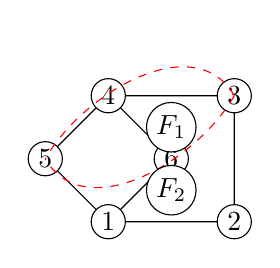
\begin{tikzpicture}[scale=0.8, every node/.style={circle, draw, fill=white, inner sep=1.5pt}]
        \coordinate (v1) at (0,0);
        \coordinate (v2) at (2,0);
        \coordinate (v3) at (2,2);
        \coordinate (v4) at (0,2);
        \coordinate (v5) at (-1,1);
        \coordinate (v6) at (1,1);
        \draw (v1)--(v2)--(v3)--(v4)--(v5)--(v1);
        \draw (v1)--(v6)--(v4);
        \node at (v1) {1};
        \node at (v2) {2};
        \node at (v3) {3};
        \node at (v4) {4};
        \node at (v5) {5};
        \node at (v6) {6};
        \draw[red, dashed] (v3) to[out=120,in=60] (v5);
        \draw[red, dashed] (v3) to[out=-120,in=-60] (v5);
        \node at (1,1.5) {$F_1$};
        \node at (1,0.5) {$F_2$};
    \end{tikzpicture}
    \caption{A biconnected plane graph with a separation pair \((3,5)\). 
    Triangulating faces \(F_1\) and \(F_2\) independently can add the chord \((3,5)\) twice, creating a multi‑edge.}
    \label{fig:separation_pair}
\end{figure}

Figure~\ref{fig:separation_pair} illustrates a biconnected graph where vertices \(3\) and \(5\) form a separation pair: removing them disconnects the graph. 
If we triangulate the outer face \(F_1\) and the inner face \(F_2\) independently using the algorithm of Parvez et al., we might add the chord \((3,5)\) in both faces, leading to a multi‑edge. 
Such multi‑edges are not allowed in simple graphs, and the algorithm would generate invalid triangulations.

Thus, a direct application of the Parvez–Rahman–Nakano algorithm to biconnected graphs fails. 
Our goal is to overcome this limitation while preserving the optimal \(O(1)\) amortized time per triangulation.

\section{Our Contribution}
\label{sec:contribution}

We present the first algorithm for generating all triangulations of a \emph{biconnected} plane graph in \(O(1)\) amortized time per triangulation and \(O(n)\) space. 
Our main innovations are:

\begin{enumerate}
    \item \textbf{Local genealogical trees:} Instead of processing all faces simultaneously, we process faces one by one in a fixed order. 
    For each face, we construct a local genealogical tree of triangulations that are compatible with previously triangulated faces.
    
    \item \textbf{Safe root vertex selection:} We introduce the concept of a \emph{safe root vertex} for a face. 
    A safe root vertex guarantees that the fan triangulation from that vertex does not create any multi‑edge with chords from previous faces. 
    We prove that every face in a biconnected plane graph contains at least two safe root vertices, regardless of the chords already present.
    
    \item \textbf{Linear‑time safe root finding:} Using a two‑pointer technique based on planarity, we find a safe root vertex in \(O(n)\) time, where \(n\) is the number of vertices in the face. 
    This ensures that the building cost per face can be amortized.
    
    \item \textbf{Valid generating set (VGS):} We maintain a set of generating chords whose flip will not create a multi‑edge. 
    When flipping a chord, only four border chords change their opposite pairs; we update the VGS in constant time using linked lists.
    
    \item \textbf{Global chord set with dynamic push/pop:} A global hash set stores all chords currently on the exploration path. 
    This allows \(O(1)\) conflict detection and supports backtracking in the recursive DFS.
    
    \item \textbf{Pruning strategy:} If a blocking chord (i.e., a chord that does not have the root vertex as an endpoint) conflicts with a chord from a previous face, all descendant triangulations are invalid. 
    We prune such branches safely, without losing any valid triangulation.
\end{enumerate}

Our algorithm achieves the same optimal complexity as the triconnected case while handling the strictly larger class of biconnected graphs.

\section{Comparison with Existing Algorithms}
\label{sec:comparison}

Table~\ref{tab:comparison} summarises the differences between our algorithm and previous work.

\begin{table}[htbp]
    \centering
    \caption{Comparison of triangulation enumeration algorithms.}
    \label{tab:comparison}
    \begin{tabular}{|l|l|c|c|}
        \hline
        \textbf{Algorithm} & \textbf{Graph Class} & \textbf{Time per triangulation} & \textbf{Space} \\
        \hline
        Reverse search~\cite{avis1996} & General & \(O(n^2)\) or worse & \(O(n)\) \\
        Li–Nakano~\cite{li2001} & Biconnected & \(O(r^2 n)\) & --- \\
        Nakano (improved) & Biconnected & \(O(r n)\) & --- \\
        Parvez et al.~\cite{parvez2011} & Triconnected & \(O(1)\) amortized & \(O(n)\) \\
        \textbf{This work} & \textbf{Biconnected} & \(\mathbf{O(1)}\) \textbf{amortized} & \(\mathbf{O(n)}\) \\
        \hline
    \end{tabular}
\end{table}

Our algorithm is the first to achieve constant amortised time for the class of biconnected plane graphs, which includes many practical instances.

\section{Thesis Organization}
\label{sec:organization}

The remainder of this thesis is structured as follows.

\begin{itemize}
    \item \textbf{Chapter 2} introduces the necessary graph‑theoretic concepts: connectivity, planarity, cycles, chords, triangulations, flipping operations, and genealogical trees. 
    Special emphasis is given to separation pairs and the distinction between triconnected and biconnected graphs.
    
    \item \textbf{Chapter 3} describes the baseline algorithm for generating all triangulations of a single cycle (the Parvez–Rahman–Nakano algorithm) in detail. 
    We present the definitions of blocking chords, generating chords, and leftmost blocking chords, and prove uniqueness.
    
    \item \textbf{Chapter 4} clarifies the distinction between our naming of the generating set and that of the original paper, and proves the condition for flipping generating chords.
    
    \item \textbf{Chapter 5} explains why the original algorithm fails for biconnected graphs due to separation pairs and the multi‑edge problem.
    
    \item \textbf{Chapter 6} introduces our pruning strategy based on the persistence of chords that do not involve the root vertex.
    
    \item \textbf{Chapter 7} presents the multi‑layer DFS that processes faces one by one, maintaining a global chord set and backtracking.
    
    \item \textbf{Chapter 8} addresses the problem of generating chords themselves causing multi‑edges and introduces the concept of safe root vertices.
    
    \item \textbf{Chapter 9} proves a lower bound of \(\Omega(n)\) triangulations per face, which is essential for amortised analysis.
    
    \item \textbf{Chapter 10} gives an \(O(n)\) two‑pointer algorithm for finding a safe root vertex.
    
    \item \textbf{Chapter 11} describes the valid generating set (VGS) and how to update it in constant time during flips.
    
    \item \textbf{Chapter 12} presents the complete algorithm in pseudocode and proves its correctness.
    
    \item \textbf{Chapter 13} analyses the time and space complexity, proving \(O(1)\) amortised time per triangulation and \(O(n)\) space.
    
    \item \textbf{Chapter 14} provides experimental validation on 35 test cases, including cycles, grids, and complex graphs, confirming the theoretical bounds.
    
    \item \textbf{Chapter 15} discusses why the algorithm cannot be extended to 1‑connected graphs in general, giving examples where safe roots do not exist.
    
    \item \textbf{Chapter 16} outlines future work, including extensions to 1‑connected graphs and 1‑planar graphs.
    
    \item \textbf{Chapter 17} concludes the thesis with a summary of contributions and final remarks.
\end{itemize}